%!TEX root = ../main.tex
\section{System Requirements} % (fold)
\label{sec:system_requirements}

\martin{The big system picture should be on its own page}

\begin{figure}[!h]
	\centering
	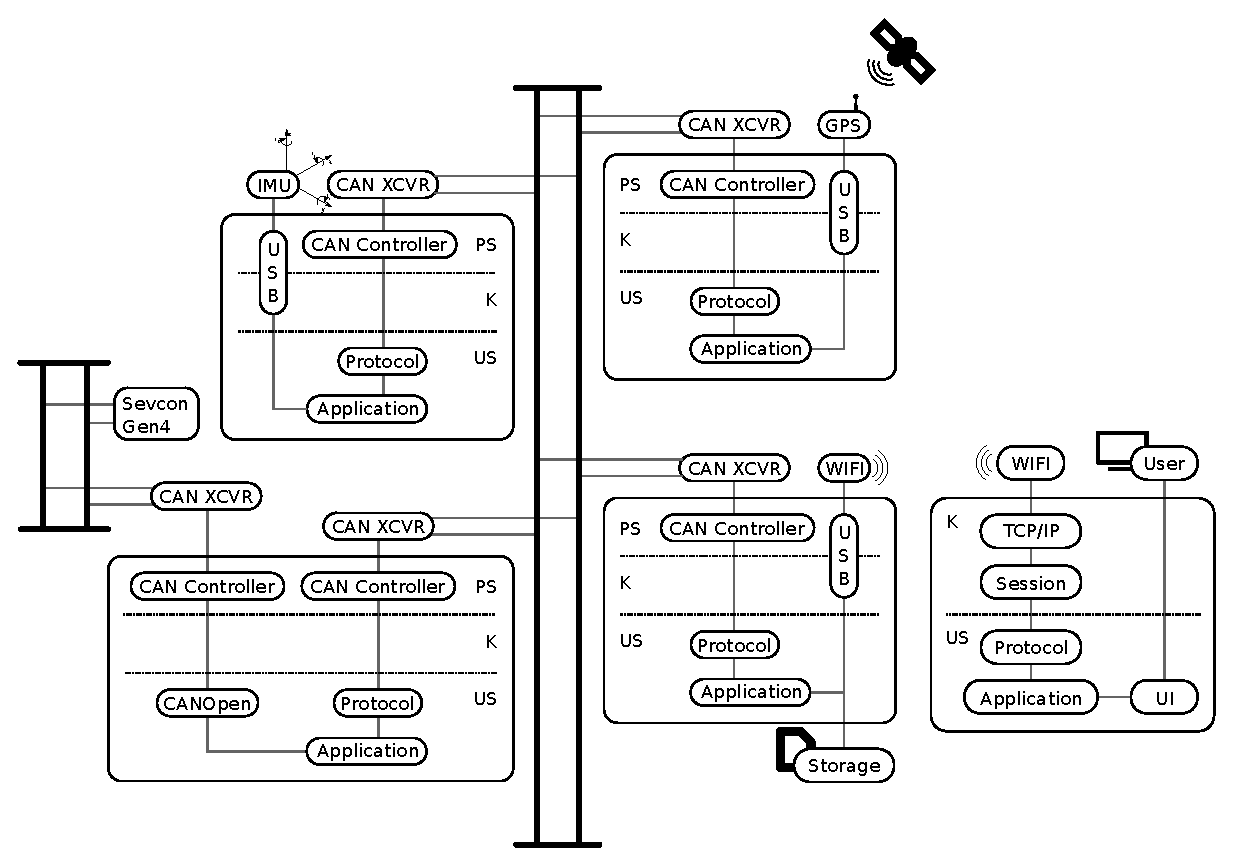
\includegraphics[angle=90,width=\textwidth]{graphics/analysis_complex.eps}
	\caption{The big system........}
	\label{fig:complete_system}
\end{figure}



\subsection{Actors}
The only actor on the system is an engineer.

\subsection{Interfaces}
\begin{itemize}
\item Wifi, for data transfer between go-kart and stationary computer.
\item CAN bus, for local network.
\item CanOpen, for interfacing the Sevcon.
\item USB, for GPS and IMU.
\item ??, for SD card connection.
\item Powersupply, for Zybo boards.
\end{itemize}

\subsection{Functional requirements}
The system: 
\begin{itemize}
\item Reads data from sensors.
\item Reads data from Sevcon.
\item Transfers data to stationary computer using Wifi.
\item Presents data to the user.
\item Logs sensordata to SD card.
\item Read data from SD card.
\item Timestamps all data. 
\end{itemize}

\subsection{Operational requirements}
The system monitors go-kart data.% when engineer starts the system by powering it on.

\subsection{Quality of service requirements}
\begin{itemize}
\item IMU data must be sampled with xx Hz.
\item GPS data must be sampled with zz Hz.
\item Data logging with qq Hz.??
\end{itemize}

\subsection{Parametric requirements}
Wifi range must be greater than xx meters.

\subsection{Design requirements}
The system:
\begin{itemize}
\item must be scalable to at least 16 sensors/nodes.
\item must be modular to allow easy integration of new sensors/nodes.
\item must be functional if one or more sensors/nodes stop working.	 
\end{itemize}


% section system_requirements (end)